\section{Numerical validation and orbital reconstruction}
\label{sec:numerics}

\subsection{Numerical strategy}

The numerical tests are based on the exact local return of the reduced flow.  Critical-jet predictions are fixed before comparison with periodic-orbit observables.  The action is evaluated from the exact section formula
\[
\mcJ=\frac12\int_\Gamma(F^*\lambda-\lambda),
\qquad \lambda=q\,dp,
\]
so that the very small residual actions do not require subtraction of two large flow integrals.  The implementation and convergence diagnostics are described in \cref{app:numerics}.

\subsection{Multiprecision localization of the resonant primary orbit}

A dedicated high-order Taylor integrator was used to repeat the resonance computation in arbitrary precision.  The trigonometric state equations and the variational equations are advanced by recursively generated Taylor coefficients, so the calculation does not rely on double-precision ODE arithmetic.

The refined resonant parameter is
\begin{equation}
\boxed{
\mu_\star
=0.66286900693051012809369086386036365\ldots
}
\label{eq:mustar-mp}
\end{equation}
with
\[
y_\star
=-2.57258930747694896652177432487053\ldots,
\]
\[
T_{1/4,\star}
=3.01795545336085961004746139780291\ldots.
\]

At 120-digit working precision, using a Taylor order of 38 and maximal step size $0.05$, the complete event-corrected monodromy satisfies
\[
\boxed{
\|DP_{\mu_\star}+I\|_F
\simeq 6.24\times10^{-47},
}
\]
while
\[
|\det DP_{\mu_\star}-1|
\simeq1.89\times10^{-49}.
\]
The residual off-diagonal entries are at the $10^{-47}$ scale or smaller.  This convergence of the complete matrix, rather than the trace alone, is the numerical basis for identifying the resonance as semisimple.

\subsection{Independent critical-jet re-extraction}

The complete fifth-order return jet was re-extracted independently in multiprecision by transporting a bivariate polynomial jet in the section variables $(q,p)$ through the Taylor integrator.  The variable return time is then solved formally, degree by degree, from the implicit event equation $x(T_\star+\tau(q,p),q,p)=0$.  This avoids polynomial regression of sampled map values.

The nonlinear oddification is fixed by the nonresonant gauge described in \cref{app:normal-form}: a cubic Hamiltonian generator removes the quadratic map term and a quintic generator removes the quartic map term, with no additional resonant quartic generator.  Two independent transports, using $h_{\max}=0.22$ at 55-digit working precision and $h_{\max}=0.20$ at 60-digit working precision, give a stable sextic plateau.

The linear and quartic balancing scales are
\[
\boxed{
\alpha_{\rm lin}=0.0946271414514,\qquad
\alpha_{\rm bal}=0.0946271414515,
}
\]
with relative discrepancy approximately $1.2\times10^{-12}$.  In the fixed reversible chart the re-extracted coefficients are
\[
A=203.6723580,\qquad B=-408.3087120,
\]
\[
\rho=2.001182918,\qquad
\sigma=-4.7330723\times10^{-3},
\]
and
\[
d=27009.26240,\qquad e=271555.83499,
\]
\[
f=512441.22879,\qquad g=75140.77917.
\]
Hence
\[
\boxed{
G=886147.10535,\qquad
\Delta_6=-289016.91057.
}
\]
The two jet discretizations differ by only $3.0\times10^{-6}$ in $d$, $1.8\times10^{-5}$ in $e$, $1.6\times10^{-5}$ in $f$, and $1.6\times10^{-7}$ in $g$ in absolute units; the resulting values of $G$ differ by $1.4\times10^{-6}$.  The corresponding scalar crossover scale is
\[
\deltax\simeq1.0486840\times10^{-6}.
\]
These quantities are fixed before comparison with the periodic-orbit observables below.

\subsection{Axial action law and orbital quartic calibration}

The leading axial normal form predicts
\[
\mcJ_H=-\frac{\delta^2}{16A}+\bigO(\delta^3),
\]
so that
\begin{equation}
\boxed{
A_{\rm orb}(\delta)
=-\frac{\delta^2}{16\bar{\mcJ}},
\qquad
\bar{\mcJ}=\frac{\mcJ_Q+\mcJ_P}{2}.
}
\label{eq:Aorb}
\end{equation}
The physical second-return exponents similarly give
\begin{equation}
\boxed{
\rho_{\rm orb}(\delta)
=
\frac{\kappa_{F,Q}+\kappa_{F,P}}{4\delta}.
}
\label{eq:rhoorb}
\end{equation}

The exact-return results from two interlaced dyadic ladders are shown in \cref{tab:orbital-quartic}.  The raw estimators approach the critical-jet values monotonically as $\delta$ decreases.

\begin{table}[t]
\centering
\caption{Orbital reconstruction of the leading quartic coefficients from exact axial period-two orbits.}
\label{tab:orbital-quartic}
\begin{tabular}{ccc}
\toprule
$\delta$ & $A_{\rm orb}$ & $\rho_{\rm orb}$ \\
\midrule
$2.0\times10^{-2}$ & $202.35030$ & $2.0103251$ \\
$1.0\times10^{-2}$ & $203.00736$ & $2.0058993$ \\
$5.0\times10^{-3}$ & $203.33850$ & $2.0035771$ \\
$1.6\times10^{-2}$ & $202.61225$ & $2.0085900$ \\
$8.0\times10^{-3}$ & $203.13954$ & $2.0049791$ \\
$4.0\times10^{-3}$ & $203.40492$ & $2.0031040$ \\
\bottomrule
\end{tabular}
\end{table}

First Richardson extrapolation gives, on the successive pairs of the two ladders,
\[
A_{\rm orb}^{[1]}
=203.66441,
\ 203.66964,
\ 203.66683,
\ 203.67029,
\]
and
\[
\rho_{\rm orb}^{[1]}
=2.0014734,
\ 2.0012549,
\ 2.0013681,
\ 2.0012289.
\]
These values converge toward
\[
A_{\rm jet}=203.6723580,
\qquad
\rho_{\rm jet}=2.001182918.
\]
Thus the quartic balance, and in particular the proximity to $\rho=2$, is visible directly in invariant periodic-orbit observables rather than only in the fitted return jet.

\subsection{Why the subleading axial coefficients do not isolate the critical sextic jet}
\label{sec:axial-contamination}

The numerical campaign also exposes an important limitation of the simpler axial reconstruction proposed at an earlier stage of the analysis.  The detuned normal form has the structure
\begin{equation}
K_\delta
=
-\delta I
+H_4
+H_6
+\delta\,H_{4,1}
+\gamma\delta^2 I
+\cdots,
\label{eq:detuned-extended}
\end{equation}
where $H_{4,1}$ is a detuning-dependent quartic polynomial.  On an axial branch, $I=\bigO(\delta)$, and therefore
\[
H_6=\bigO(\delta^3),
\qquad
\delta H_{4,1}=\bigO(\delta^3),
\qquad
\delta^2 I=\bigO(\delta^3).
\]
Consequently, the $\delta^3$ action coefficient and the $\delta^2$ Floquet correction contain both the critical sextic jet and detuning-dependent lower-order terms.  They cannot be used to reconstruct $d,e,f,g$ from the critical map alone unless the parameter-dependent normal form is computed to the same order.

This is confirmed by the exact-return data: the two axial families have the correct common leading law $2\rho\delta$, but their measured subleading Floquet corrections do not agree with formulas containing only the critical coefficients $d,e,f,g$.  We therefore use the axial branches only for the robust leading reconstruction of $A$ and $\rho$.  No sextic coefficient is inferred from the contaminated subleading axial channel in the final analysis.

\subsection{Elliptic action reconstruction of \texorpdfstring{$G$}{G}}

The near-diagonal branch provides a cleaner test of the sextic coefficient.  Within the scalar reduction,
\[
3\mcJ_E=aI^2-2\delta I,
\]
so the physical positive root is
\[
I
=
\frac{
\delta-\sqrt{\delta^2+3a\mcJ_E}
}{a},
\]
and
\begin{equation}
\boxed{
G_{\rm ell}
=
\frac{\delta-2aI}{3I^2}.
}
\label{eq:Gell}
\end{equation}

The reconstruction is remarkably stable throughout the inner crossover region.  Representative values are
\begin{table}[t]
\centering
\caption{Elliptic action reconstruction of $G$.  The fixed critical-jet target is $G_{\rm jet}=8.8614711\times10^5$.}
\label{tab:Gell}
\begin{tabular}{ccc}
\toprule
$u=\delta/\deltax$ & $G_{\rm ell}$ & relative difference from $G_{\rm jet}$ \\
\midrule
$0$    & $8.85903\times10^5$ & $-2.8\times10^{-4}$ \\
$0.01$ & $8.86023\times10^5$ & $-1.4\times10^{-4}$ \\
$0.1$  & $8.85904\times10^5$ & $-2.8\times10^{-4}$ \\
$1$    & $8.85186\times10^5$ & $-1.1\times10^{-3}$ \\
$10$   & $8.82339\times10^5$ & $-4.3\times10^{-3}$ \\
$100$  & $8.73139\times10^5$ & $-1.47\times10^{-2}$ \\
\bottomrule
\end{tabular}
\end{table}
The gradual outer drift is consistent with higher-order corrections becoming more visible as the branch leaves the local crossover scale.

\subsection{Residual elliptic period-two cycles at resonance}

At $\mu=\mu_\star$, direct multiprecision solution of
\[
F(q,p)=(q,p)
\]
finds the nonzero residual period-two cycles predicted by the sixth-order normal form.  One representative fixed point of $F$ is
\[
\boxed{
(q,p)
=
(2.56839185346349\times10^{-4},
 2.83395697372187\times10^{-3})
}
\]
and its first-return companion is
\[
P(q,p)
=
(-2.67259191745878\times10^{-4},
 -2.70365354787740\times10^{-3}).
\]
The second symmetry-related cycle supplies the other two nonzero fixed points of $F$.

The physical second-return Floquet angle is
\[
\boxed{
\vartheta_F
=1.62684506536\times10^{-4},
}
\]
with
\[
\tr DF
=1.99999997353375139\ldots,
\]
and the multiprecision determinant error is below $10^{-23}$ in this computation.

The exact reduced symplectic action is
\begin{equation}
\boxed{
\mcJ_0^{\rm exact}
=-1.69102354131\times10^{-13}.
}
\label{eq:residual-action-exact}
\end{equation}
For comparison, the scalar prediction is
\[
\mcJ_0^{\rm scalar}
=-1.69009171482\times10^{-13},
\]
while the sixth-order polynomial prediction is approximately
\[
\mcJ_0^{(6)}
=-1.69021\times10^{-13}.
\]
The residual exact action is therefore already reproduced at the $10^{-3}$ level by the frozen sixth-order description.

\subsection{Direct quartic--sextic crossover}
\label{sec:numerical-crossover}

The exact elliptic family was continued through
\[
u=0,\ 0.01,\ 0.03,\ 0.1,\ 0.3,\ 1,\ 3,\ 10,\ 30,\ 100.
\]
The branch was selected by continuation from the residual cycle together with the sixth-order predictor; this avoids numerical jumps to the coexisting axial fixed points at the largest detunings.

For the invariant normalized action and Floquet angle,
\[
Y=\frac{\mcJ_E}{\mcJ_0^{\rm scalar}},
\qquad
Z=\frac{\vartheta_F}{\vartheta_0^{\rm scalar}},
\]
the exact-return data closely follow the coefficient-independent scalar curves
\[
Y_{\rm sc}=4R^3-3R^2,
\qquad
Z_{\rm sc}=R\sqrt{2R-1}.
\]
Representative comparisons are shown in \cref{tab:crossover-data}.

\begin{table}[t]
\centering
\caption{Exact-return crossover compared with the scalar prediction.}
\label{tab:crossover-data}
\begin{tabular}{ccccc}
\toprule
$u$ & $Y$ & $Y_{\rm sc}$ & $Z$ & $Z_{\rm sc}$ \\
\midrule
$0$    & $1.00055$ & $1.00000$ & $0.99997$ & $1.00000$ \\
$0.01$ & $1.04545$ & $1.04517$ & $1.01494$ & $1.01492$ \\
$0.1$  & $1.46679$ & $1.46611$ & $1.14267$ & $1.14263$ \\
$1$    & $6.75730$ & $6.74997$ & $2.12186$ & $2.12132$ \\
$10$   & $109.605$ & $109.300$ & $7.75513$ & $7.74866$ \\
$30$   & $504.342$ & $502.040$ & $16.2990$ & $16.2759$ \\
$100$  & $2859.51$ & $2836.57$ & $38.3127$ & $38.2148$ \\
\bottomrule
\end{tabular}
\end{table}

Across this entire range the normalized action differs from the scalar curve by less than $0.81\%$, and the normalized Floquet angle by less than $0.52\%$.  The data therefore connect the residual plateau continuously to the outer sextic regime without any fitted crossover parameter.

The independent critical-jet audit also reconstructs the nonlinear canonical chart.  Writing
\[
I_{\rm NF}=\frac{Q^2+P^2}{2},
\qquad
X=\frac{I_{\rm NF}}{I_0^{\rm scalar}},
\]
the exact-return amplitude follows the scalar prediction $X_{\rm sc}=R(u)$ to within $0.62\%$ over the full range $0\le u\le100$.  At the residual cycle, $X=1.00037$, a deviation of only $0.037\%$ from the scalar plateau.  Reconstructing the canonical map with the two independent jet discretizations changes $I_{\rm NF}$ by at most $4.0\times10^{-13}$ relatively across the entire crossover.  The first-return companion points have equal $I_{\rm NF}$ to relative accuracy better than $7\times10^{-6}$ even at $u=100$.

\begin{figure}[t]
\centering
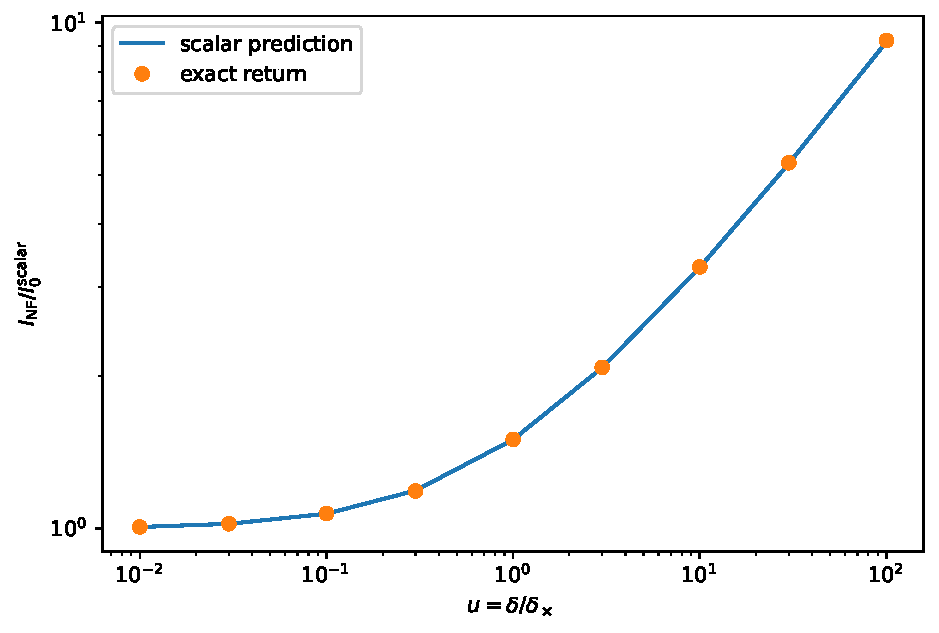
\includegraphics[width=.72\linewidth]{figures/fig06_amplitude_crossover.pdf}
\caption{Normal-form amplitude across the quartic--sextic crossover.  Exact-return fixed points are transformed with the independently reconstructed critical canonical chart.  The continuous curve is the coefficient-independent scalar prediction $X=R(u)$; no amplitude normalization is fitted to the continuation data.}
\label{fig:amplitude-crossover}
\end{figure}

Eliminating $u$ gives an additional parameter-free test.  The exact data remain close to
\[
Y=4X^3-3X^2,\qquad Z=X\sqrt{2X-1}.
\]
The maximum relative departures over the computed range are about $1.1\%$ in the action relation and $0.7\%$ in the Floquet relation.

\begin{figure}[t]
\centering
\begin{subfigure}{.48\linewidth}
\centering
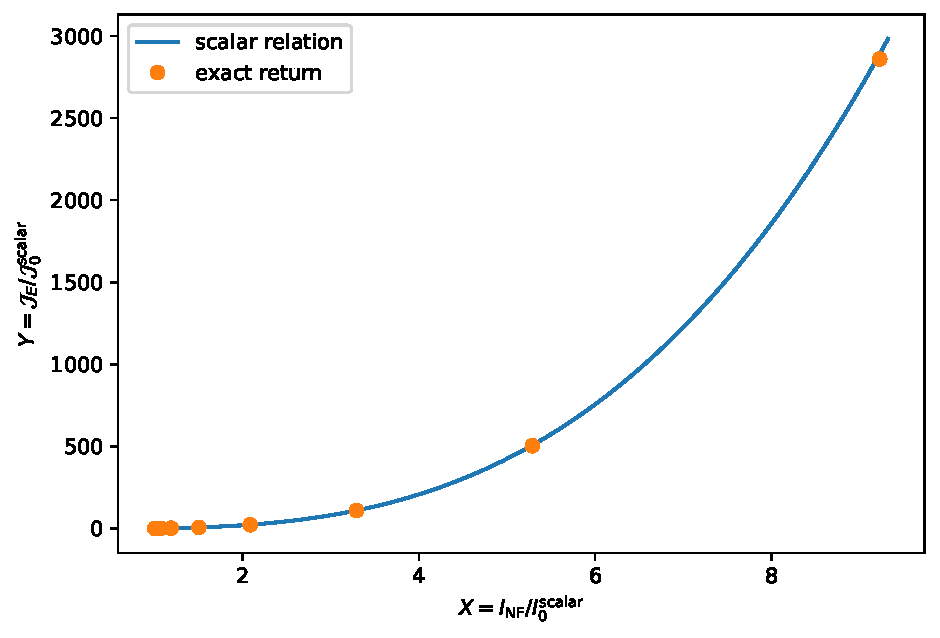
\includegraphics[width=\linewidth]{figures/fig08_action_vs_amplitude.pdf}
\caption{Action--amplitude relation.}
\end{subfigure}
\hfill
\begin{subfigure}{.48\linewidth}
\centering
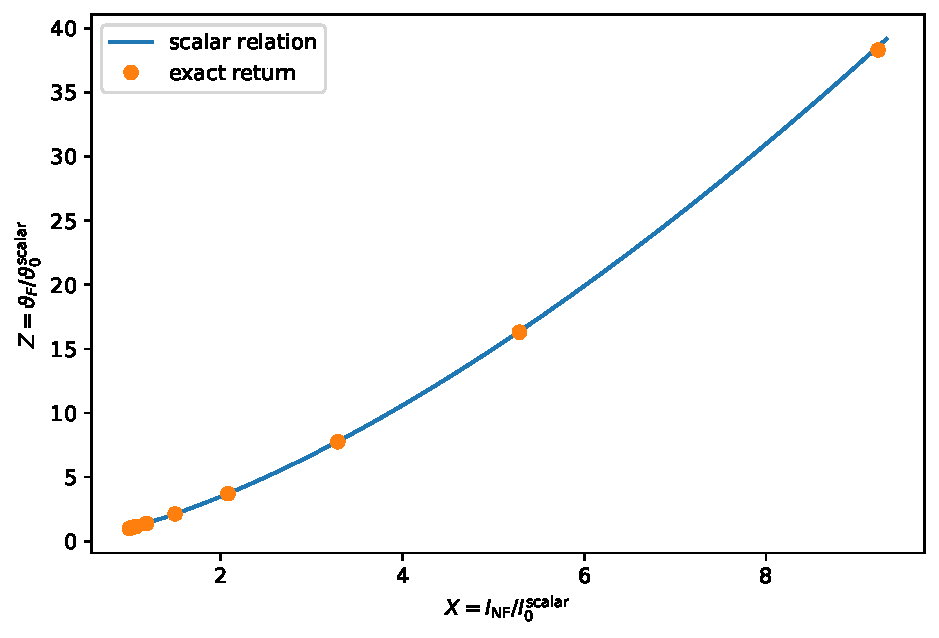
\includegraphics[width=\linewidth]{figures/fig08_floquet_vs_amplitude.pdf}
\caption{Floquet--amplitude relation.}
\end{subfigure}
\caption{Parameter-free crossover tests after eliminating the continuation parameter.  The curves are the scalar relations; the markers are exact-return observables in the reconstructed canonical chart.}
\label{fig:parameter-free}
\end{figure}

\subsection{Effective exponents}

Local logarithmic slopes extracted from neighboring continuation points track the scalar effective exponents.  For example, near $u=1$ the discrete data give
\[
\nu_{\mcJ}\simeq0.968,
\qquad
\nu_\vartheta\simeq0.426,
\]
compared with the scalar values
\[
1,
\qquad
\frac7{16}=0.4375.
\]
By $u=30$ the agreement is much tighter:
\[
\nu_{\mcJ}\simeq1.41646
\quad\text{versus}\quad
1.41703,
\]
\[
\nu_\vartheta\simeq0.69375
\quad\text{versus}\quad
0.69484.
\]
The observed drift toward $3/2$ and $3/4$ confirms the intermediate-asymptotic interpretation rather than a fixed power law extending to resonance.


\begin{figure}[t]
\centering
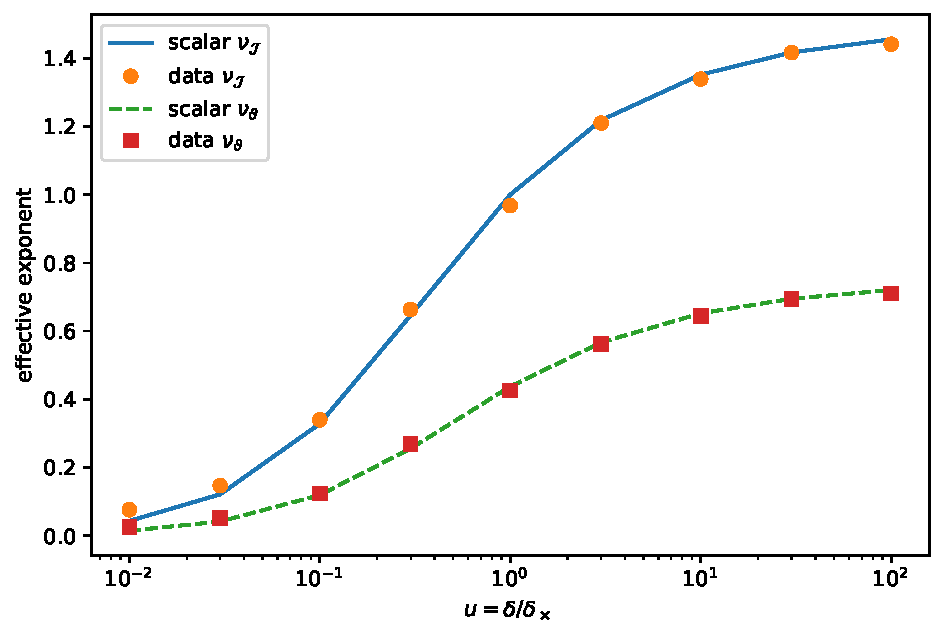
\includegraphics[width=.72\linewidth]{figures/fig07_effective_exponents.pdf}
\caption{Effective action and Floquet exponents across the exact-return crossover, compared with the scalar prediction.}
\label{fig:effective-exponents}
\end{figure}

\begin{figure}[t]
\centering
\begin{subfigure}{.48\linewidth}
\centering
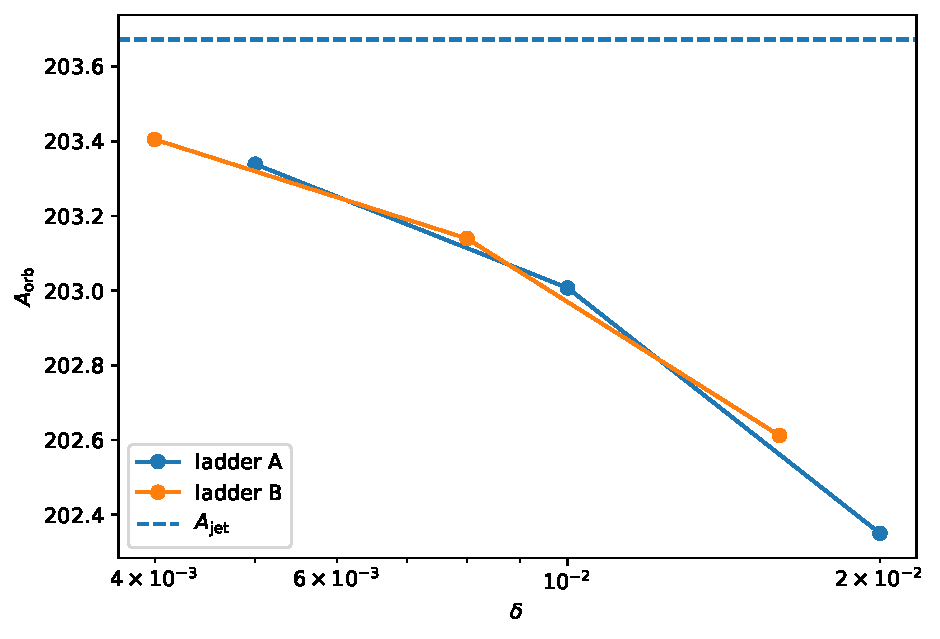
\includegraphics[width=\linewidth]{figures/fig09_Aorb.pdf}
\caption{Orbital reconstruction of $A$.}
\end{subfigure}
\hfill
\begin{subfigure}{.48\linewidth}
\centering
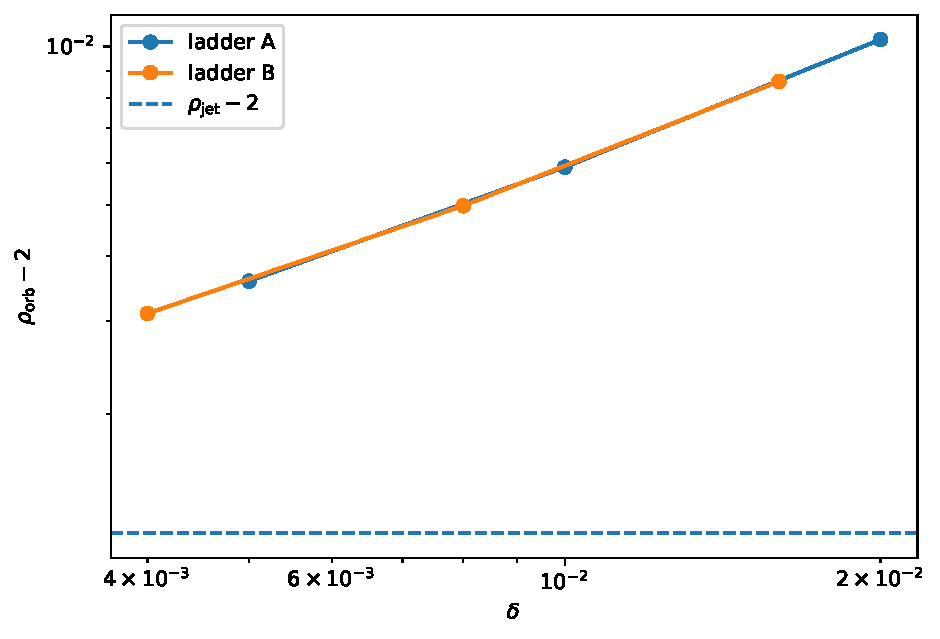
\includegraphics[width=\linewidth]{figures/fig09_rhoorb_minus2.pdf}
\caption{Orbital reconstruction of $\rho-2$.}
\end{subfigure}
\caption{Leading quartic coefficients reconstructed from exact axial action and Floquet observables.  Horizontal reference lines are fixed by the independent critical-jet extraction.}
\label{fig:orbital-quartic}
\end{figure}

\subsection{Numerical status}

The following parts of the numerical program are now complete:
\begin{itemize}[leftmargin=2em]
\item multiprecision localization and semisimplicity audit of the $1{:}2$ resonance;
\item independent multiprecision transport of the complete critical fifth-order return jet;
\item canonical nonresonant oddification and reconstruction of $H_4$, $H_6$, and the nonlinear normal-form chart;
\item exact-return axial validation of the leading quartic coefficients $A$ and $\rho$;
\item multiprecision residual-cycle action and Floquet calculation;
\item exact-return crossover continuation from $u=0$ to $u=100$, including the normal-form amplitude $I_{\rm NF}$;
\item elliptic action reconstruction of the diagonal sextic coefficient $G$;
\item parameter-free amplitude--action and amplitude--Floquet crossover tests.
\end{itemize}

The campaign also shows that a sextic reconstruction from subleading axial coefficients alone is not justified without the detuning-dependent normal form in \eqref{eq:detuned-extended}; this claim has therefore been removed rather than fitted away.  The principal remaining extension is no longer required for the present conclusions: it would be the full parameter-dependent normal form through the weighted order needed to separate critical sextic and detuning-dependent contributions on the axial branches.
